\documentclass[]{article}
\usepackage{lmodern}
\usepackage{amssymb,amsmath}
\usepackage{ifxetex,ifluatex}
\usepackage{fixltx2e} % provides \textsubscript
\ifnum 0\ifxetex 1\fi\ifluatex 1\fi=0 % if pdftex
  \usepackage[T1]{fontenc}
  \usepackage[utf8]{inputenc}
\else % if luatex or xelatex
  \ifxetex
    \usepackage{mathspec}
  \else
    \usepackage{fontspec}
  \fi
  \defaultfontfeatures{Ligatures=TeX,Scale=MatchLowercase}
\fi
% use upquote if available, for straight quotes in verbatim environments
\IfFileExists{upquote.sty}{\usepackage{upquote}}{}
% use microtype if available
\IfFileExists{microtype.sty}{%
\usepackage{microtype}
\UseMicrotypeSet[protrusion]{basicmath} % disable protrusion for tt fonts
}{}
\usepackage[margin=1in]{geometry}
\usepackage{hyperref}
\hypersetup{unicode=true,
            pdftitle={P8105\_hw1\_sim2128},
            pdfauthor={Sarah Munro},
            pdfborder={0 0 0},
            breaklinks=true}
\urlstyle{same}  % don't use monospace font for urls
\usepackage{color}
\usepackage{fancyvrb}
\newcommand{\VerbBar}{|}
\newcommand{\VERB}{\Verb[commandchars=\\\{\}]}
\DefineVerbatimEnvironment{Highlighting}{Verbatim}{commandchars=\\\{\}}
% Add ',fontsize=\small' for more characters per line
\usepackage{framed}
\definecolor{shadecolor}{RGB}{248,248,248}
\newenvironment{Shaded}{\begin{snugshade}}{\end{snugshade}}
\newcommand{\AlertTok}[1]{\textcolor[rgb]{0.94,0.16,0.16}{#1}}
\newcommand{\AnnotationTok}[1]{\textcolor[rgb]{0.56,0.35,0.01}{\textbf{\textit{#1}}}}
\newcommand{\AttributeTok}[1]{\textcolor[rgb]{0.77,0.63,0.00}{#1}}
\newcommand{\BaseNTok}[1]{\textcolor[rgb]{0.00,0.00,0.81}{#1}}
\newcommand{\BuiltInTok}[1]{#1}
\newcommand{\CharTok}[1]{\textcolor[rgb]{0.31,0.60,0.02}{#1}}
\newcommand{\CommentTok}[1]{\textcolor[rgb]{0.56,0.35,0.01}{\textit{#1}}}
\newcommand{\CommentVarTok}[1]{\textcolor[rgb]{0.56,0.35,0.01}{\textbf{\textit{#1}}}}
\newcommand{\ConstantTok}[1]{\textcolor[rgb]{0.00,0.00,0.00}{#1}}
\newcommand{\ControlFlowTok}[1]{\textcolor[rgb]{0.13,0.29,0.53}{\textbf{#1}}}
\newcommand{\DataTypeTok}[1]{\textcolor[rgb]{0.13,0.29,0.53}{#1}}
\newcommand{\DecValTok}[1]{\textcolor[rgb]{0.00,0.00,0.81}{#1}}
\newcommand{\DocumentationTok}[1]{\textcolor[rgb]{0.56,0.35,0.01}{\textbf{\textit{#1}}}}
\newcommand{\ErrorTok}[1]{\textcolor[rgb]{0.64,0.00,0.00}{\textbf{#1}}}
\newcommand{\ExtensionTok}[1]{#1}
\newcommand{\FloatTok}[1]{\textcolor[rgb]{0.00,0.00,0.81}{#1}}
\newcommand{\FunctionTok}[1]{\textcolor[rgb]{0.00,0.00,0.00}{#1}}
\newcommand{\ImportTok}[1]{#1}
\newcommand{\InformationTok}[1]{\textcolor[rgb]{0.56,0.35,0.01}{\textbf{\textit{#1}}}}
\newcommand{\KeywordTok}[1]{\textcolor[rgb]{0.13,0.29,0.53}{\textbf{#1}}}
\newcommand{\NormalTok}[1]{#1}
\newcommand{\OperatorTok}[1]{\textcolor[rgb]{0.81,0.36,0.00}{\textbf{#1}}}
\newcommand{\OtherTok}[1]{\textcolor[rgb]{0.56,0.35,0.01}{#1}}
\newcommand{\PreprocessorTok}[1]{\textcolor[rgb]{0.56,0.35,0.01}{\textit{#1}}}
\newcommand{\RegionMarkerTok}[1]{#1}
\newcommand{\SpecialCharTok}[1]{\textcolor[rgb]{0.00,0.00,0.00}{#1}}
\newcommand{\SpecialStringTok}[1]{\textcolor[rgb]{0.31,0.60,0.02}{#1}}
\newcommand{\StringTok}[1]{\textcolor[rgb]{0.31,0.60,0.02}{#1}}
\newcommand{\VariableTok}[1]{\textcolor[rgb]{0.00,0.00,0.00}{#1}}
\newcommand{\VerbatimStringTok}[1]{\textcolor[rgb]{0.31,0.60,0.02}{#1}}
\newcommand{\WarningTok}[1]{\textcolor[rgb]{0.56,0.35,0.01}{\textbf{\textit{#1}}}}
\usepackage{graphicx,grffile}
\makeatletter
\def\maxwidth{\ifdim\Gin@nat@width>\linewidth\linewidth\else\Gin@nat@width\fi}
\def\maxheight{\ifdim\Gin@nat@height>\textheight\textheight\else\Gin@nat@height\fi}
\makeatother
% Scale images if necessary, so that they will not overflow the page
% margins by default, and it is still possible to overwrite the defaults
% using explicit options in \includegraphics[width, height, ...]{}
\setkeys{Gin}{width=\maxwidth,height=\maxheight,keepaspectratio}
\IfFileExists{parskip.sty}{%
\usepackage{parskip}
}{% else
\setlength{\parindent}{0pt}
\setlength{\parskip}{6pt plus 2pt minus 1pt}
}
\setlength{\emergencystretch}{3em}  % prevent overfull lines
\providecommand{\tightlist}{%
  \setlength{\itemsep}{0pt}\setlength{\parskip}{0pt}}
\setcounter{secnumdepth}{0}
% Redefines (sub)paragraphs to behave more like sections
\ifx\paragraph\undefined\else
\let\oldparagraph\paragraph
\renewcommand{\paragraph}[1]{\oldparagraph{#1}\mbox{}}
\fi
\ifx\subparagraph\undefined\else
\let\oldsubparagraph\subparagraph
\renewcommand{\subparagraph}[1]{\oldsubparagraph{#1}\mbox{}}
\fi

%%% Use protect on footnotes to avoid problems with footnotes in titles
\let\rmarkdownfootnote\footnote%
\def\footnote{\protect\rmarkdownfootnote}

%%% Change title format to be more compact
\usepackage{titling}

% Create subtitle command for use in maketitle
\providecommand{\subtitle}[1]{
  \posttitle{
    \begin{center}\large#1\end{center}
    }
}

\setlength{\droptitle}{-2em}

  \title{P8105\_hw1\_sim2128}
    \pretitle{\vspace{\droptitle}\centering\huge}
  \posttitle{\par}
    \author{Sarah Munro}
    \preauthor{\centering\large\emph}
  \postauthor{\par}
    \date{}
    \predate{}\postdate{}
  

\begin{document}
\maketitle

\begin{Shaded}
\begin{Highlighting}[]
\KeywordTok{library}\NormalTok{(tidyverse)}
\end{Highlighting}
\end{Shaded}

\begin{verbatim}
## -- Attaching packages ----------------------------------------- tidyverse 1.2.1 --
\end{verbatim}

\begin{verbatim}
## v ggplot2 3.2.1     v purrr   0.3.2
## v tibble  2.1.3     v dplyr   0.8.3
## v tidyr   0.8.3     v stringr 1.4.0
## v readr   1.3.1     v forcats 0.4.0
\end{verbatim}

\begin{verbatim}
## -- Conflicts -------------------------------------------- tidyverse_conflicts() --
## x dplyr::filter() masks stats::filter()
## x dplyr::lag()    masks stats::lag()
\end{verbatim}

\begin{Shaded}
\begin{Highlighting}[]
\KeywordTok{library}\NormalTok{(tibble)}
\end{Highlighting}
\end{Shaded}

\#Problem 1

\begin{Shaded}
\begin{Highlighting}[]
\KeywordTok{set.seed}\NormalTok{(}\DecValTok{10}\NormalTok{)}
\NormalTok{hw1_df =}\StringTok{ }\KeywordTok{tibble}\NormalTok{(}
  \DataTypeTok{sharks =} \KeywordTok{rnorm}\NormalTok{(}\DecValTok{8}\NormalTok{),}
  \DataTypeTok{positive =}\NormalTok{ sharks }\OperatorTok{>}\StringTok{ }\DecValTok{0}\NormalTok{, }
  \DataTypeTok{species =} \KeywordTok{c}\NormalTok{(}\StringTok{"White"}\NormalTok{, }\StringTok{"Tiger"}\NormalTok{, }\StringTok{"Nurse"}\NormalTok{, }\StringTok{"Bull"}\NormalTok{, }\StringTok{"Whale"}\NormalTok{, }\StringTok{"Lemon"}\NormalTok{, }\StringTok{"Hammerhead"}\NormalTok{,   }\StringTok{"Mako"}\NormalTok{),}
  \DataTypeTok{aggression =} \KeywordTok{factor}\NormalTok{(}\KeywordTok{c}\NormalTok{(}\StringTok{"High"}\NormalTok{, }\StringTok{"High"}\NormalTok{, }\StringTok{"Low"}\NormalTok{, }\StringTok{"High"}\NormalTok{, }\StringTok{"Low"}\NormalTok{, }\StringTok{"High"}\NormalTok{, }\StringTok{"Medium"}\NormalTok{, }\StringTok{"Medium"}\NormalTok{))}
\NormalTok{)}

\KeywordTok{mean}\NormalTok{(}\KeywordTok{pull}\NormalTok{(hw1_df, sharks))}
\end{Highlighting}
\end{Shaded}

\begin{verbatim}
## [1] -0.3779272
\end{verbatim}

\begin{Shaded}
\begin{Highlighting}[]
\CommentTok{#The mean was taken properly}
\KeywordTok{mean}\NormalTok{(}\KeywordTok{pull}\NormalTok{(hw1_df, positive))}
\end{Highlighting}
\end{Shaded}

\begin{verbatim}
## [1] 0.375
\end{verbatim}

\begin{Shaded}
\begin{Highlighting}[]
\CommentTok{#The mean was taken properly}
\KeywordTok{mean}\NormalTok{(}\KeywordTok{pull}\NormalTok{(hw1_df, species))}
\end{Highlighting}
\end{Shaded}

\begin{verbatim}
## Warning in mean.default(pull(hw1_df, species)): argument is not numeric or
## logical: returning NA
\end{verbatim}

\begin{verbatim}
## [1] NA
\end{verbatim}

\begin{Shaded}
\begin{Highlighting}[]
\CommentTok{#The mean was unable to be taken}
\KeywordTok{mean}\NormalTok{(}\KeywordTok{pull}\NormalTok{(hw1_df, aggression))}
\end{Highlighting}
\end{Shaded}

\begin{verbatim}
## Warning in mean.default(pull(hw1_df, aggression)): argument is not numeric
## or logical: returning NA
\end{verbatim}

\begin{verbatim}
## [1] NA
\end{verbatim}

\begin{Shaded}
\begin{Highlighting}[]
\CommentTok{#The mean was unable to be taken}
\end{Highlighting}
\end{Shaded}

\begin{Shaded}
\begin{Highlighting}[]
\CommentTok{#Convert the logical vector to a numeric vector}
\KeywordTok{as.numeric}\NormalTok{(}\KeywordTok{pull}\NormalTok{(hw1_df, positive))}
\CommentTok{#Convert the character vector to a numeric vector}
\KeywordTok{as.numeric}\NormalTok{(}\KeywordTok{pull}\NormalTok{(hw1_df, species))}
\CommentTok{#Convert the factor vector to a numeric vector}
\KeywordTok{as.numeric}\NormalTok{(}\KeywordTok{pull}\NormalTok{(hw1_df, aggression))}

\CommentTok{#You can convert the logical and factor vectors to numeric, but you are unable to covert the character vector to numeric. This would explain why the mean of the character variable cannot be taken, the characters do not correspond to any numeric values. }
\end{Highlighting}
\end{Shaded}

\begin{Shaded}
\begin{Highlighting}[]
\CommentTok{#Convert the logical vector to a numeric vector, then multiply the random sample by the result}
\KeywordTok{as.numeric}\NormalTok{(}\KeywordTok{pull}\NormalTok{(hw1_df, positive))}\OperatorTok{*}\NormalTok{(}\KeywordTok{pull}\NormalTok{(hw1_df, sharks))}
\end{Highlighting}
\end{Shaded}

\begin{verbatim}
## [1] 0.01874617 0.00000000 0.00000000 0.00000000 0.29454513 0.38979430
## [7] 0.00000000 0.00000000
\end{verbatim}

\begin{Shaded}
\begin{Highlighting}[]
\CommentTok{#Convert the logical vector to a factor vector, then multiply the random sample by the result}
\KeywordTok{as.factor}\NormalTok{(}\KeywordTok{pull}\NormalTok{(hw1_df, positive))}\OperatorTok{*}\NormalTok{(}\KeywordTok{pull}\NormalTok{(hw1_df, sharks))}
\end{Highlighting}
\end{Shaded}

\begin{verbatim}
## Warning in Ops.factor(as.factor(pull(hw1_df, positive)), (pull(hw1_df,
## sharks))): '*' not meaningful for factors
\end{verbatim}

\begin{verbatim}
## [1] NA NA NA NA NA NA NA NA
\end{verbatim}

\begin{Shaded}
\begin{Highlighting}[]
\CommentTok{#Convert the logical vector to a factor factor, then convert the result to numeric, then multiply the random sample by the result}
\KeywordTok{as.numeric}\NormalTok{(}\KeywordTok{as.factor}\NormalTok{(}\KeywordTok{pull}\NormalTok{(hw1_df, positive)))}\OperatorTok{*}\NormalTok{(}\KeywordTok{pull}\NormalTok{(hw1_df, sharks))}
\end{Highlighting}
\end{Shaded}

\begin{verbatim}
## [1]  0.03749234 -0.18425254 -1.37133055 -0.59916772  0.58909025  0.77958860
## [7] -1.20807618 -0.36367602
\end{verbatim}

\begin{Shaded}
\begin{Highlighting}[]
\CommentTok{#The result was not meaningful for the factors, they were assigned values of NA}
\end{Highlighting}
\end{Shaded}

\#Problem 2

\begin{Shaded}
\begin{Highlighting}[]
\KeywordTok{set.seed}\NormalTok{(}\DecValTok{500}\NormalTok{)}
\NormalTok{part2_df =}\StringTok{ }\KeywordTok{tibble}\NormalTok{(}
  \DataTypeTok{x =} \KeywordTok{rnorm}\NormalTok{(}\DecValTok{500}\NormalTok{),}
  \DataTypeTok{y =} \KeywordTok{rnorm}\NormalTok{(}\DecValTok{500}\NormalTok{),}
  \DataTypeTok{logicv =}\NormalTok{ x }\OperatorTok{+}\StringTok{ }\NormalTok{y }\OperatorTok{>}\StringTok{ }\DecValTok{1}\NormalTok{,}
  \DataTypeTok{numberv =} \KeywordTok{as.numeric}\NormalTok{(logicv),}
  \DataTypeTok{factorv =} \KeywordTok{as.factor}\NormalTok{(numberv)}
\NormalTok{)}
\end{Highlighting}
\end{Shaded}

The dataset \texttt{part2\_df1} has 500 rows and 5 columns. The mean of
x is -0.0455615, the median is -0.0385267, and the standard deviation is
1.0165813. The proportion of \texttt{logicv} for which x + y
\textgreater{} 1 is 0.22

\begin{Shaded}
\begin{Highlighting}[]
\CommentTok{#Scatter plot with colors corresponding to the logical vector}
\KeywordTok{ggplot}\NormalTok{(part2_df, }\KeywordTok{aes}\NormalTok{(}\DataTypeTok{x =}\NormalTok{ x, }\DataTypeTok{y =}\NormalTok{ y, }\DataTypeTok{color=}\NormalTok{logicv)) }\OperatorTok{+}\StringTok{ }\KeywordTok{geom_point}\NormalTok{()}
\end{Highlighting}
\end{Shaded}

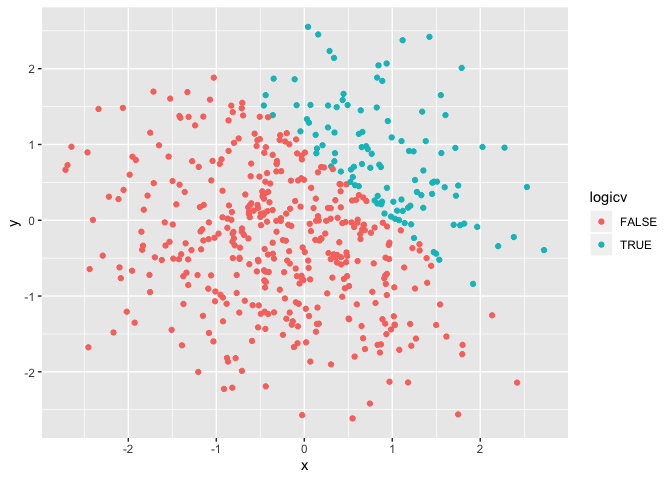
\includegraphics{P8105_hw1_sim2128_files/figure-latex/unnamed-chunk-6-1.pdf}

\begin{Shaded}
\begin{Highlighting}[]
\KeywordTok{ggsave}\NormalTok{(}\StringTok{"scatter_plot1.pdf"}\NormalTok{)}
\end{Highlighting}
\end{Shaded}

\begin{verbatim}
## Saving 6.5 x 4.5 in image
\end{verbatim}

\begin{Shaded}
\begin{Highlighting}[]
\CommentTok{#Scatter plot with colors corresponding to the numeric vector}
\KeywordTok{ggplot}\NormalTok{(part2_df, }\KeywordTok{aes}\NormalTok{(}\DataTypeTok{x =}\NormalTok{ x, }\DataTypeTok{y =}\NormalTok{ y, }\DataTypeTok{color=}\NormalTok{numberv)) }\OperatorTok{+}\StringTok{ }\KeywordTok{geom_point}\NormalTok{()}
\end{Highlighting}
\end{Shaded}

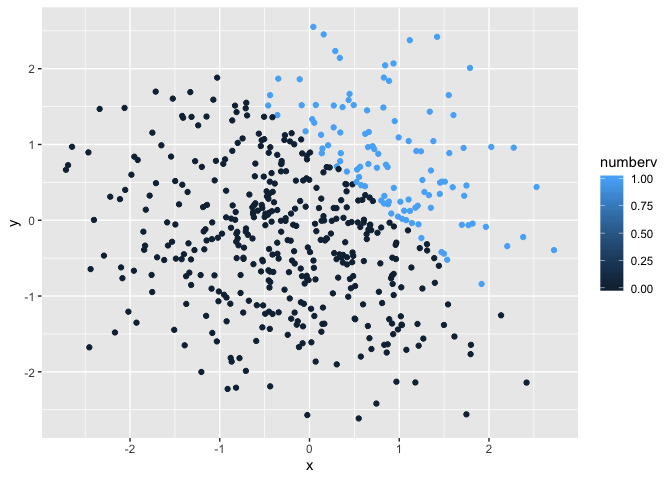
\includegraphics{P8105_hw1_sim2128_files/figure-latex/unnamed-chunk-6-2.pdf}

\begin{Shaded}
\begin{Highlighting}[]
\CommentTok{#Scatter plot with colors corresponding to the factor vector}
\KeywordTok{ggplot}\NormalTok{(part2_df, }\KeywordTok{aes}\NormalTok{(}\DataTypeTok{x =}\NormalTok{ x, }\DataTypeTok{y =}\NormalTok{ y, }\DataTypeTok{color=}\NormalTok{factorv)) }\OperatorTok{+}\StringTok{ }\KeywordTok{geom_point}\NormalTok{()}
\end{Highlighting}
\end{Shaded}

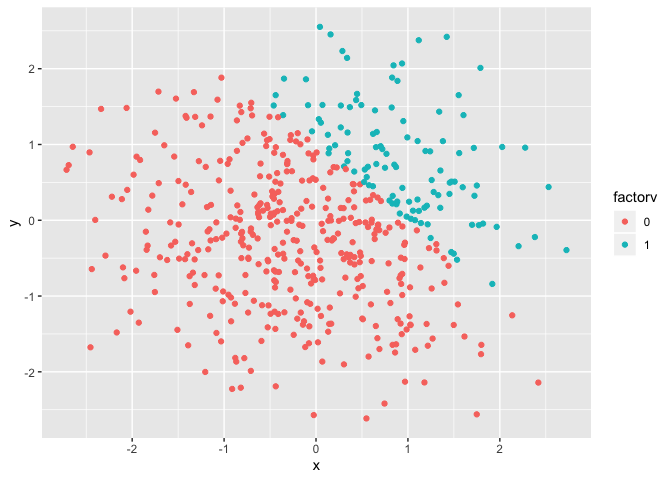
\includegraphics{P8105_hw1_sim2128_files/figure-latex/unnamed-chunk-6-3.pdf}

\begin{Shaded}
\begin{Highlighting}[]
\CommentTok{#The distribution appeared the same for all three plots. The colors appeared the same only for the plots corresponding to the logical and factor vector. For the plot with colors corresponding to the numeric vector, there was a scale of color rather than 2 single options of red or blue. }
\end{Highlighting}
\end{Shaded}


\end{document}
